\documentclass[]{article}
\usepackage{lmodern}
\usepackage{amssymb,amsmath}
\usepackage{ifxetex,ifluatex}
\usepackage{achicago}

\usepackage{fixltx2e} % provides \textsubscript
\ifnum 0\ifxetex 1\fi\ifluatex 1\fi=0 % if pdftex
  \usepackage[T1]{fontenc}
  \usepackage[utf8]{inputenc}
\else % if luatex or xelatex
  \ifxetex
    \usepackage{mathspec}
  \else
    \usepackage{fontspec}
  \fi
  \defaultfontfeatures{Mapping=tex-text,Scale=MatchLowercase}
  \newcommand{\euro}{€}
\fi
% use upquote if available, for straight quotes in verbatim environments
\IfFileExists{upquote.sty}{\usepackage{upquote}}{}
% use microtype if available
\IfFileExists{microtype.sty}{%
\usepackage{microtype}
\UseMicrotypeSet[protrusion]{basicmath} % disable protrusion for tt fonts
}{}
\makeatletter
\@ifpackageloaded{hyperref}{}{%
\ifxetex
  \usepackage[setpagesize=false, % page size defined by xetex
              unicode=false, % unicode breaks when used with xetex
              xetex]{hyperref}
\else
  \usepackage[unicode=true]{hyperref}
\fi
}
\@ifpackageloaded{color}{
    \PassOptionsToPackage{usenames,dvipsnames}{color}
}{%
    \usepackage[usenames,dvipsnames]{color}
}
\usepackage[top=1in, bottom=1.25in, left=1in, right=1in]{geometry}

\usepackage{titling}

\setlength{\droptitle}{-5em} 

\usepackage{listings}

\usepackage{sectsty}
\sectionfont{\fontsize{16}{16}\selectfont}
\subsectionfont{\fontsize{14}{14}\selectfont}
\subsubsectionfont{\fontsize{12}{12}\selectfont}

\renewcommand{\familydefault}{\sfdefault} 
\makeatother
\hypersetup{breaklinks=true,
            bookmarks=true,
            pdfauthor={},
            pdftitle={Title},
            colorlinks=true,
            citecolor=black,
            urlcolor=blue,
            linkcolor=magenta,
            pdfborder={0 0 0}
            }
\urlstyle{same}  % don't use monospace font for urls
\usepackage{longtable,booktabs}
\usepackage{graphicx,grffile}
\makeatletter
\def\maxwidth{\ifdim\Gin@nat@width>\linewidth\linewidth\else\Gin@nat@width\fi}
\def\maxheight{\ifdim\Gin@nat@height>\textheight\textheight\else\Gin@nat@height\fi}
\makeatother
% Scale images if necessary, so that they will not overflow the page
% margins by default, and it is still possible to overwrite the defaults
% using explicit options in \includegraphics[width, height, ...]{}
\setkeys{Gin}{width=\maxwidth,height=\maxheight,keepaspectratio}
\setlength{\parindent}{0pt}
\setlength{\parskip}{6pt plus 2pt minus 1pt}
\setlength{\emergencystretch}{3em}  % prevent overfull lines
\providecommand{\tightlist}{%
  \setlength{\itemsep}{0pt}\setlength{\parskip}{0pt}}
\setcounter{secnumdepth}{0}

\title{Title}
\date{}

% Redefines (sub)paragraphs to behave more like sections
\ifx\paragraph\undefined\else
\let\oldparagraph\paragraph
\renewcommand{\paragraph}[1]{\oldparagraph{#1}\mbox{}}
\fi
\ifx\subparagraph\undefined\else
\let\oldsubparagraph\subparagraph
\renewcommand{\subparagraph}[1]{\oldsubparagraph{#1}\mbox{}}
\fi

\begin{document}
\maketitle
\vspace*{-8em}

\begin{center}
Name Surname\textsuperscript{1}, Name Surname\textsuperscript{2}, and
Name
Surname\textsuperscript{2}

\textsuperscript{1} Author affiliation, Town, Country

Author email

\textsuperscript{2} Author affiliation, Town, Country

Author 2 email

Author 3 email

\end{center}

\textbf{Abstract.} Summarize the contents of the paper in 100 to 150 words.

\textbf{Keywords:} Separated by commas.

\section{Introduction}\label{introduction}

Format all text using the styles. The final document for publication should be delivered in PDF format.

\section{Preparation of the Document}\label{preparation-of-the-document}

Author's names should not include academic titles or descriptions. Names of multiple authors should be separated with commas. Affiliations should
be composed below the name or list of names and include town (if it is not already part of the affiliation itself) and country. Email contacts should be listed directly below the affiliations. Multiple affiliations should be marked with superscript numbers and shown in new lines as shown in this template.

Please don't leave empty lines between paragraphs - this template already adds space between them. Format longer citations as indented paragraphs, without quotation marks, and format short citations inline with double quotes, for example, for example "human synergy with the computer could leave way for individual expression and creativity." \cite{risset890237423423487}

\begin{quote}
While some mental states, such as experiences, may be determined internally, there are other cases in which external factors make a significant contribution. In particular, we will argue that \emph{beliefs} can be constituted partly by features of the environment, when those features play the right sort of role in driving cognitive processes. If so, the mind extends into the world. \cite{Clark:1998mz}
\end{quote}

\subsection{Figures and Tables}\label{figures-and-tables}

\begin{table}[h]
\centering
\label{table1}
\begin{tabular}{|l|l|l|l|l|}
\hline
  & A  & B & C  \\ \hline
A & 10 & 1 & 1  \\ \hline
B & 3  & 7 & 2  \\ \hline
C & 5  & 1 & 1  \\ \hline
\end{tabular}
\caption{Caption: below the table}
\end{table}

Table captions should be composed below the table, and figure captions should be composed below the figures, both using the same style. All captions should be numbered sequentially and should include a reference to the source whenever necessary.

\begin{figure}[h]
\begin{center}
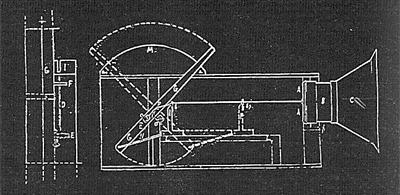
\includegraphics{Intonarumori-schema.png}
\caption{Intonarumori Schema}
\label{fig1}
\end{center}
\end{figure}

\subsection{Program Code}\label{program-code}

Program listings in the text should be set in the appropriate style.

\begin{lstlisting}
background(loadImage("rockies.jpg"));
PImage img = loadImage("degaul.jpg");
image(img, 0, 0);
blend(img, 0, 0, 33, 100, 67, 0, 33, 100, DARKEST);
\end{lstlisting}

\paragraph{Example of a pixel blend function from {\url{http://processing.org/reference/blend\_.html}}}

\subsection{Notes}\label{notes}

Superscript references to notes should be composed either directly after the word, phrase or sentence to be discussed or immediately following the punctuation mark,\footnote{This is an example of a footnote.} if applicable. Number all footnotes sequentially and do not include any footnotes in the abstract.

\subsection{Citations and
Bibliography}\label{citations-and-bibliography}

Citations in the text should be labelled with (Author Year) or (Author Year, page) following the Chicago Manual of Style conventions. For example, \cite{Wilson:1998dz} or \cite[27]{auslander2008liveness}. The references section should be organised alphabetically and chronologically. All references should be written in the Latin alphabet and where applicable list the original language at the end of the transcription or translation of the title, e.g., (in Chinese) or (in Greek).

The author-date Chicago-Style Citation Quick Guide can be accessed online at {\url{http://www.chicagomanualofstyle.org/tools\_citationguide.html}}

\section{Headings}\label{headings}

Compose all headings the appropriate styles.  Section headings are 16pt bold.

\subsection{Subheadings}

Subheadings are 14pt bold.

\subsubsection{Subsubheadings}

Subsubheadings are 12pt bold.

\section{Additional Information}\label{additional-information}

The submission of the final version of the article constitutes an authorisation for its publishing in the \textbf{International Conference on Live Interfaces 2016} proceedings.

\textbf{Acknowledgements.} If necessary they should always be composed with a run-in heading formatted in bold, and placed at the end of the text prior to the references.

  \bibliographystyle{achicago}
  \bibliography{test.bib}

\end{document}
